\section{Results and discussion}

Figure \ref{fig:top5} shows the top 5 best images (here we choose the first 5 images from the ranked training set) retrieved for 2 query images. For the first query image, images with the shades of white tops and block bottoms are retrieved. For the second query image, images with V-neck tops/dresses are retrieved. Figure \ref{fig:Bottom_5} shows the worst 5 images (here we choose the last 5 images from the ranked training set) for 2 query images. We observe that images retrieved seen in figure \ref{fig:top5} have the least Euclidean distance of the embedding with respect to the query image. As seen in figure \ref{fig:Bottom_5}, we observe that retrieved images have the maximum Euclidean distance of the embedding with respect to query image.


Figure \ref{fig:orig} shows one of the images obtained from the Image Ranking model. We provide an option to change the color of the apparel of the image obtained. Figure \ref{fig:result1} shows the result obtained after switching the color of the apparel to the desired color of the user. Figure \ref{fig:result2} shows the segmented image of the apparel that will be useful in generating the dataset required for Image segmentation


% \begin{figure}%
%     \centering
%     \subfloat[label 1]{{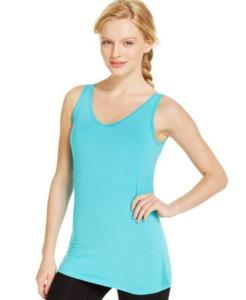
\includegraphics[width=6cm]{imgs/orig.jpg} }}%
%     \qquad
%     \subfloat[label 2]{{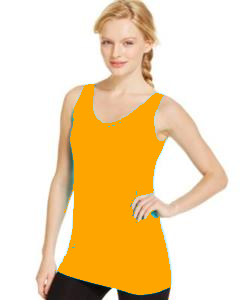
\includegraphics[width=6cm]{imgs/result1.png} }}%
%     \caption{2 Figures side by side}%
%     \label{fig:gulati}%
% \end{figure}



\begin{figure}
\begin{subfigure}{0.1\textwidth}
\includegraphics[width=\linewidth]{imgs}
\caption{First subfigure} \label{fig:1a}
\end{subfigure}
\hspace*{\fill} % separation between the subfigures
\begin{subfigure}{0.1\textwidth}
\includegraphics[width=\linewidth]{fig_b.pdf}
\caption{Second subfigure} \label{fig:1b}
\end{subfigure}
\caption{A figure that contains three subfigures} \label{fig:1}
\end{figure}


